\begin{center}
\footnotesize\noindent\fbox{
	\parbox{\textwidth}{
	  Utilizzare il metodo di Jacobi per risolvere il sistema lineare
	  $$
	  A_n \textbf{x} = \begin{pmatrix} 1 \\ \vdots \\ 1 \end{pmatrix}
	  $$

	  dove $A_n$ è la matrice definita nell'Esercizio 1, con tolleranza $tol=10^{-5}$, e partendo dal vettore nullo. Graficare il numero di iterazioni necessarie, rispetto alla dimensione $n$ del problema, con $n$ che varia da 100 a 1000 (con passo 20).
}
}\end{center}

\begin{center}
	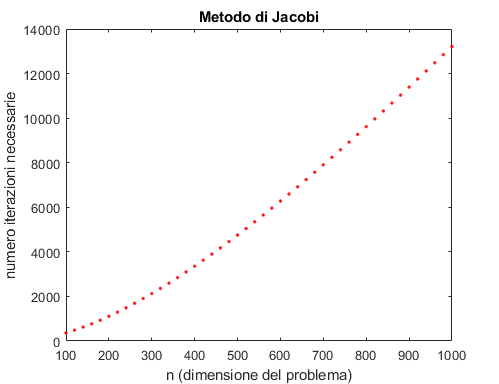
\includegraphics[scale=0.9]{cap6/6_3.png}
\end{center}

\noindent Il codice Matlab utilizzato per realizzarle il grafico mostrato \'e il seguente: \\

\lstinputlisting[language=Matlab]{cap6/6_3.m}
